\section{Anatomical Joint Coordinate Systems}
\label{sec:4_CoordSys}

In this section, we are interested in a completely different application than the previous ones, though it is also aimed at validating the correspondence relations quality of the generated meshes \mr*. We propose the computation of a joint coordinate system for the trapezio\-metacarpal (TMC) joint. Joint coordinate systems are a common tool for the analysis of joint kinematics. They are composed of two coordinate systems, one attached to each bone of the joint. The description of a motion is based on the rigid movement of the distal bone with respect to the proximal one. We are concerned with the TMC joint, the articulation situated at the base of the thumb, connecting the trapezium and the \first* metacarpal, as shown in \figref{im:4_TPM_location}. But we argue that once the method has been proven reliable for this joint, it can naturally be transferred to any other wrist articulation. 

The computation of anatomical coordinate systems offers a dual benefit for our work:
our method is completely based on the correspondence relations between the meshes $M_{W,\{b,i\}}$ previously computed. The quality of the results fully depend on the quality of the corresponding points locations. We prove that we get equivalent results to another analytical specialized approach, we therefore consider it an evidence that the corresponding meshes are to be trusted. Additionally, our method is general and naturally functional for any other joint. We illustrate that the database that has been put in correspondence can have many applications in various domains. While in the previous sections we were focused on shape models for 3D shape registration, we are now concerned with a biomechanical utilization. 


\subsection{State of the art}


The unique versatility of the human hand is due to its opposable thumb, essential for dexterity as well as for effective handling \cite{jones_2006_human}. These skills rely on the thumb's large range of motion \cite{cooney_1981_kinesiology}, enabled mostly by the trapeziometacarpal joint . % ([?]).
This articulation is also one of the joints the most affected by osteoarthritis \cite{marshall_2010_radiographic}, 
which can prove to be disabling in everyday life. 
For these reasons, it is important to study the thumb and the TMC joint. 
Several previous works have addressed the TMC joint kinematics (\cite{halilaj_2014_vivo}, \cite{crisco_2015_vivo}, \cite{kawanishi_2018_vivo}). It is an intricate joint, composed of saddle-shaped articular surfaces, as shown in \figref{im:4_TPM_surface_articulation}. The two main mechanical axes for extension-flexion and abduction-adduction are nonorthogonal and nonintersecting (\cite{hollister_1992_axes}, \cite{crisco_2015_vivo}). 
%It is important to continue to study the joint and have a better comprehension of it, as it might help diagnose and treat thumb afflictions such as osteoarthritis.

Studies of joints motions require the definition of geometrical reference systems in order to describe the bones kinematics. A strong condition to define such a system is the necessity of reproducibility. Multiple reference systems for the TMC have been proposed in the literature, as more appropriate systems allow to be more precise in the kinematics description. In particular, axes parallel to the direction of movement are ideal, though they are also required to be easily reproducible. %One joint system is composed of two coordinates systems, one for each of the bones forming the articulation.

Cooney et al. \cite{cooney_1981_kinesiology} were among the first ones to propose a joint reference system for the TMC. The definition of the system is based on the location of anatomical landmarks identified during a cadaver study. It is composed of a fixed coordinate system on the trapezium and a moving one on the $1^{st}$ metacarpal. In \cite{wu_1995_isb}, the International Society of Biomechanics (ISB) issued global recommendations on the definition of joint coordinate systems. In \cite{wu_2005_isb} the ISB proposed system definitions for the joints of the human upper body, among which the wrist and the TMC joint. The axes of the carpal bones are to be parallel with the ones of the radius. The TMC joint coordinate system is defined separately: it is to be the same as the one proposed by Cooney et al \cite{cooney_1981_kinesiology}, but the axes order is changed. 
 
Cheze et al. \cite{cheze_2009_joint} refined the ISB system, their axes becoming more coherent with the thumb main degrees of freedom. However their joint reference systems are still based on anatomical landmarks and are thus subjected to variability for their identification. Variability due to landmark identification was studied by Della Croce et al. \cite{della_2005_human}. They addressed the errors made through the selection of landmarks and reported their effects on the reliability and interpretation of joint kinematics. They advise for the use of more robust methods, based on automatic image processing for instance.

Coburn et al. \cite{coburn_2007_coordinate} introduced automatically computed coordinates systems for all wrist bones, based on the bones inertial axis arranged in order of ascending inertial magnitude. While easily reproducible, these axis are dependent on the bones global shape, and might be subjects to variations on the axis directions across wrists. Typically, a change of shape away from a joint surface may influence the location of the axes, making them less representative of the joint morphology. These axis also don't follow the ISB recommendations \cite{wu_1995_isb}. 

The latest proposal for TMC joint coordinate system computation is a semi-automated method introduced by Halilaj et al. \cite{halilaj_2013_thumb}. It is based on the saddle-shaped articular geometry of the TMC joint (\figref{im:4_TPM_surface_articulation}). The articular surfaces of the trapezium and $1^{st}$ metacarpal are manually selected, then fit with fifth order polynomial surfaces. Using the approximation, the principal directions of curvature of the articular surfaces are computed. The coordinate systems origins are the two saddle points, one on each bone. The axis are oriented along the principal directions of curvature of the saddles. The polynomial approximation and the definition of the axis from the principal directions of curvature make the method very specific to local geometry and the saddle-shaped articulation. At the same time, it has been proven that the actual kinematic rotation axis for extension-flexion and for abduction-adduction movements are not always the main directions of curvature of the saddle (\cite{hollister_1992_axes}, \cite{crisco_2015_vivo}).


We propose an alternative approach of axis computation based on correspondence between meshes. The joint coordinate system is the one defined by Halilaj et al. \cite{halilaj_2013_thumb}, based on the geometry of the articular surfaces of the articulation. We show that similar performances as \cite{halilaj_2013_thumb} are achieved for the TMC joint, while having some additional benefit. Typically, the approach has the advantage of being easily adapted to any other system definition on any bone.  No limitations to inertial description or local surface approximation allows definition of truly mechanically meaningful coordinates systems. However, we focus on the TMC joint because a comparison can be drawn with the proven approach of \cite{halilaj_2013_thumb}. We evaluate the anatomical relevance of the correspondence mapping method for the TMC joint thanks to a comparison to \cite{halilaj_2013_thumb}.
%We propose a global and fully automated approach of coordinate systems definition, based on dense correspondence of the bones meshes. This technique maps all corresponding anatomical parts across bones, enabling the description and reproducibility of any coordinate system across any population. Using our method, we compute the same joint coordinate systems as \cite{halilaj_2013_thumb} and prove that we have the same precision as them. In the same time, our method has the advantage of being independent of the articular surface geometry, and can be generalized to any bones, as presented in the Discussion part. We also make possible the definition of any axis direction, in particular ones that are coherent with experimental kinematics observations. 



% The complex organization of the carpal bones leads to elaborate movements around each other to perform global wrist motions. It makes the understanding and characterization of motions complicated, as each bone can have up to 6 degrees of freedom. 
% Defining coordinates systems for some or every bones is a common
% solution to describe and measure bones kinematics (\cite{belsole_1991_carpal}, \cite{moojen_2002_three},
% \cite{coburn_coordinate_2007}, \cite{halilaj_2013_thumb}, \cite{hillstrom_2014_development}, etc...). % [Pleins d'articles qui utilisent des sys de coord en fait, combien en citer? ] 
% A strong condition to define such a system is the necessity of reproducibility from one wrist to another. The International Society of Biomechanics characterized carpal coordinates systems to be parallel to the radius system when the wrist is at rest \citep{wu_2005_isb}. 
% \cite{coburn_coordinate_2007} argued that information on the variations in carpal postures is lost with such a description and therefore proposed carpal bone coordinates systems based on the inertial axis of the bones. However these axis are dependent on the bones shapes, and might be subjects to variations on the axis directions across wrists. They also are not always the most relevant systems. 
% For instance the motion of the thumb is influenced by the articular geometry of the thumb carpometacarpal (CMC) joint. Thus \cite{halilaj_2013_thumb} introduced two systems for the trapezium and first metacarpal, according to the principal directions of curvature of the local 3D articular surfaces, inherently aligned with the primary directions of motion at the joint. 
 


% This mapping of the bones through dense correspondence can have other applications. For instance, once the points where ligaments are attached to wrist bones are localized, these locations are naturally transferred from one subject to another. 
% Or else, it allows the analysis of bone shape variation across subjects. We did explore this application through the use of a comprehensive mathematical model, a 3D Statistical Shape Model (SSM) of the human wrist. Such a model captures the distinctive features of each wrist, while offering an easy way to analyze the main modes of shape variation across the database. 
% It provides two main contributions.
% Firstly, by construction, the SSM encodes the 3D shape of wrist bones in a low dimensional space, enabling a more compact description. 
% %This encoding also eases the classification of wrists into subcategories, if those exist. 






% _________________________________________________________________________
% 					Joint Coordinate System
% _________________________________________________________________________

\subsection{Coordinate System Computation}

One of the key condition for joint coordinate systems definition is the reproducibility. It is therefore expected that if a system is defined for one instance of a shape class, we should be able to define the anatomically corresponding system on all other instances. Previous methods were either based on landmarks \cite{cooney_1981_kinesiology, wu_2005_isb}, but it is a source of variability \cite{della_2005_human}, or based on analytical analysis of the shapes \cite{halilaj_2013_thumb}. Our method reproducibility capacity rests on correspondence between shapes. 

We work with the meshes \mw*, for which we have already computed correspondence relations (Chap. \ref{chap:Method}). They are such that each $k^{th}$ vertex of bone $b$ mesh is localized on the same anatomical point of the class across the instances (\secref{ssec:2_DenseCorr_def}). Our method expects at least one instance of a coordinate system to be known originally. Then the example(s) is(are) transferred to all other instances:  

The \textit{origin of the system} is a point on the shape surface. It is either a vertex of the mesh, or a point of one of the mesh faces. In the case of a unique example, if the origin point is a vertex on the example shape, then the same vertex is the origin of the systems for all instances. It stems from the mesh correspondence properties that they are anatomically equivalent. If the example origin point is on one of the faces, its relative position on this face is computed. All origins are then located in the same position of this face, relatively to the face vertices. In the case of multiple examples, we expect the origins to be either all on the same face, or at least to be on neighboring faces. Otherwise, it would mean that the examples are already anatomically dissimilar. Let $t_R$ be the triangular face on which the most centers are. $t_R$ defines for each mesh a plane onto which the example centers are projected, the projection coordinates being expressed relatively to $t_R$ vertices.
The mean projected coordinates determine the coordinate system's center relatively to $t_R$ vertices, and can be computed for every other database subjects. 

The \textit{directions of the system} can be computed based on various properties. It can either rest on the correspondence property of the meshes, similarly to the origin definition. The directions are expressed relatively to the plane defined by the face the origin belongs to. These orientations are copied for all other coordinate systems. In the case of multiple original examples, the average orientation is transferred. Or their computation can more generally rely on global properties of 3D meshes. For instance, Halilaj et al have to approximate the shape of the articulation surface to compute the principal directions of curvature. Yet curvature tensors could also be estimated from the mesh surface (\cite{cohen_2003_restricted}) to compute the principal directions of curvature, once the saddle point has been defined. 

Our method requires no other knowledge than at least one example of a system, when the database is in correspondence. Such an example can be algorithmically computed or be given by a user. The definition is free of a mathematical or algorithmic description that must work in all cases, and is independent of landmarks. It can therefore be customized to match as well as possible the actual biomechanical axis of rotation, which are not exactly the main directions of curvature of the articulation surface in the case of the TMC joint. The results can be improved by inputting multiple examples, to limit the potential errors made both during the definition (external to our method) and the transfer phases. It is therefore recommended to define numerous example systems, though one is theoretically enough.



\subsection{Comparison with Halilaj's results}
\label{ssec:4_comparison_halilaj}


In \cite{halilaj_2013_thumb}, Halilaj et al. introduced a joint coordinate system for the TMC articulation. It is composed of two coordinates systems called Segment Coordinate Systems (SCS) defined on the trapezium (\tpm*) and the first metacarpal (\mcu*) bones. We compare the results of the SCS computation using their analytic procedure (that we call A-SCS) with our own method, based on mesh coherence across the subjects (named M-SCS). 

To test our method, annotated saddle points were needed to learn the average location. We have used the \soc* computed with Halilaj et al. method for 15 randomly chosen subjects for both articular surfaces of the \tpm* and \mcu* as training set. From these examples, we estimated the M-SCS locations for all database meshes. Multiple options were viable for the directions computation. However, we are mostly interested in the evaluation of the correspondence quality between the meshes, and therefore chose to rely on the correspondence property for the axis calculation. Similarly to the sytem location, the system orientation is computed based on the training set of 15 wrists computed with Halilaj's method.
The orientations of the example SCSs relatively to the mesh surface are transferred to the other subjects. 

As in \cite{halilaj_2013_thumb}, the evaluation is made with respect to the steadiness of the M-SCS systems origins and orientations across the database. The database bones were all affinely aligned using ICP. Inter-subject variability is defined as the difference between individual M-SCS's locations and the average one, as well as the difference of orientation between each axis and the average one. Additionally to Halilaj's paper, we measure a global angle between each individual system and the average one. It provides more information than 3 rotation angles around the $x$, $y$ and $z$ axis. This global angle is the angle of rotation around the helical axis describing the relative motion between a system and the average one. The SCS systems using the analytical method were also computed, and we compare the results of the two approaches. The evaluation of the systems steadiness is not a perfect measure to validate the accuracy of the coordinate systems. Part of the instability is due to the differences of shape of the bones and not to the method. However no ideal error metric exists to separate the shape variability from the method variability. We propose a comparison of two methods on the same shapes.


The difference of location and orientation between individual and average M-SCS systems are presented in \tabref{table:inter-subject_variability:M-SCS}. Globally both location and orientation results are slightly better for \texttt{TPM} bones than for \texttt{MC1} ones. The mean location distances are of $0.59$ mm for \texttt{TPM}s with a maximum value of $1.15$ mm, and for \texttt{MC1}s, the mean distance is $0.76$ mm with a maximum of $1.43$ mm. The global angles between the systems orientations are $4.3$\degre on average for \texttt{TPM} bones, the highest difference being $11.7$\degre and those values are $6.1$\degre and $11.5$\degre for the \texttt{MC1} bones. 

Those values are compared with the ones obtained by computing A-SCS systems on our database. 
Both systems give results in the same order of magnitude. M-SCS gets slightly better results for the \tpm* bone, especially for the origin locations, with a mean error of $0.59$ mm versus a mean error of $0.81$ mm using A-SCS. On the opposite A-SCS get slightly better results for the \texttt{MC1} origin locations. However the orientation are steadier for both bones using the correspondence based method, while the magnitude of errors remain the same.

An example of an SCS system can be observed in \figref{fig:SCS} for both \tpm* and \mcu* bones. 


\begin{table}[ht]
	\centering
	\begin{subtable}{1\textwidth}
		\centering
		\begin{tabular}{  l  c | c | c  c  c | c  }
			
			\toprule
			& & \textbf{Location (mm)} &  \multicolumn{4}{c}{\textbf{Orientation (\degre)}} \\
			& & &  X axis & Y axis & Z axis & Global angle \\
			\midrule
			\multirow{3}{*}{\tpm*} 
			& mean & $\mathbf{0.585}$ & $\mathbf{3.477}$ & $\mathbf{3.533}$ & $\mathbf{3.241}$ & $\mathbf{4.327}$ \\ 
			& max    & $1.149$ 	&   $7.298$	& 	$11.714$	&	 $9.128$ 	& 	$11.673$	\\
			& std & \footnotesize{$0.237$} 	&   \footnotesize{$1.647$}	& 	\footnotesize{$2.056$} 	&	 \footnotesize{$1.777$} 	& 	\footnotesize{$1.961$}		\\
			& & & & & & \\
			\multirow{3}{*}{\mcu*} 
			& mean & $\mathbf{0.762}$ & $\mathbf{4.901}$ & $\mathbf{5.068}$ & $\mathbf{4.378}$ & $\mathbf{6.109}$ \\ 
			& max    & $1.434$ 	&   $8.856$	& 	$11.509$ &	 $9.072$ 	& 	$11.541$	\\
			& std & \footnotesize{$0.299$} 	&   \footnotesize{$1.979$}	& 	\footnotesize{$2.354$}	 &	 \footnotesize{$2.451$} 	& 	\footnotesize{$2.192$}		\\
			\bottomrule
			
		\end{tabular}
		\caption{SCS steadiness when computed with our correspondence-based method}\label{table:inter-subject_variability:M-SCS}
	\end{subtable}
	
	\bigskip
	\begin{subtable}{1\textwidth}
		\centering
		\begin{tabular}{  l  c | c | c  c  c | c  }
			
			\toprule
			  & & \textbf{Location (mm)} &  \multicolumn{4}{c}{\textbf{Orientation (\degre)}} \\
			  & & &  X axis & Y axis & Z axis & Global angle \\
			\midrule
			\multirow{3}{*}{\tpm*} 
			& mean & $\mathbf{0.814}$ & $\mathbf{6.293}$ & $\mathbf{5.353}$ & $\mathbf{4.864}$ & $\mathbf{6.987}$ \\ 
			& max	& $1.463$	&   $16.189$	& 	$16.589$ &	 $11.456$ 	& 	$17.086$ \\
			& std   & \footnotesize{$0.315$} &   \footnotesize{$3.455$}	& 	\footnotesize{$3.104$}	 &	 \footnotesize{$2.570$} 	& 	\footnotesize{$3.347$}	 \\
		& & & & & & \\
			\multirow{3}{*}{\mcu*} 
			& mean & $\mathbf{0.706}$ & $\mathbf{5.747}$ & $\mathbf{5.121}$ & $\mathbf{6.315}$ & $\mathbf{7.280}$ \\ 
			& max & $1.614$ 	& 	$10.773$	&	$10.468$	&	$11.091$	&	$12.425$	\\
			& std & \footnotesize{$0.334$}	& 	\footnotesize{$2.885$} 	& 	\footnotesize{$2.351$}		&	\footnotesize{$2.932$}		&	\footnotesize{$2.782$}		\\
			\bottomrule
			
		\end{tabular}
		\caption{SCS steadiness when computed with \cite{halilaj_2013_thumb} analytical method}\label{table:inter-subject_variability:A-SCS}
	\end{subtable}
	\caption[Joint coordinate systems steadiness across the database]{Comparison between the analytical method of \cite{halilaj_2013_thumb} and ours : study of the inter-subject variability of the joint coordinate systems location and orientation for the \tpm* and \mcu* bones.  }
	\label{table:inter-subject_variability}
\end{table}


\begin{figure}[] 
	
	\begin{subfigure}[b]{0.45\textwidth}
		\centering
		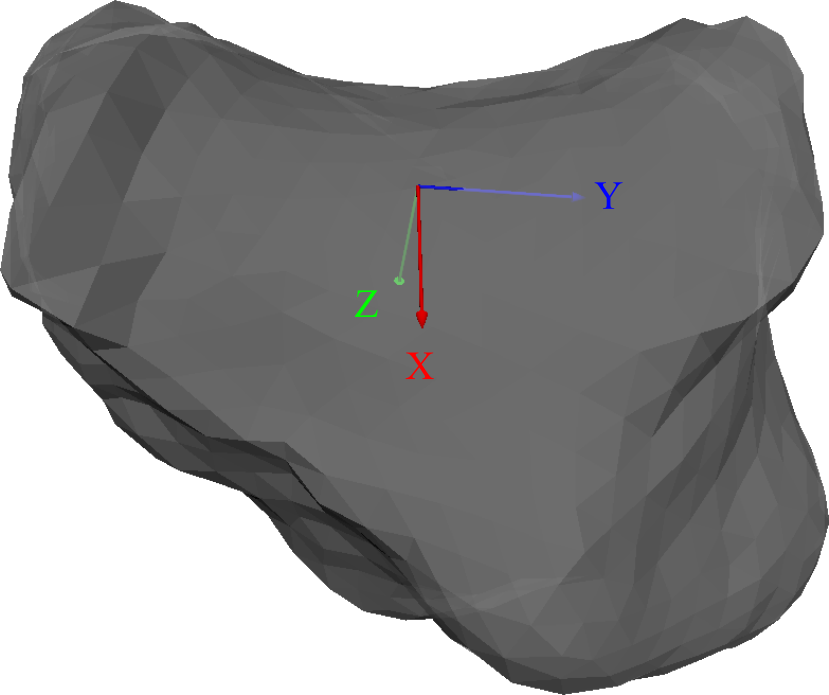
\includegraphics[width=\textwidth]{\RootDir{img/acs_tpm.png}}
	\end{subfigure}%%
	\hfill
	\begin{subfigure}[b]{0.48\linewidth}
		\centering
		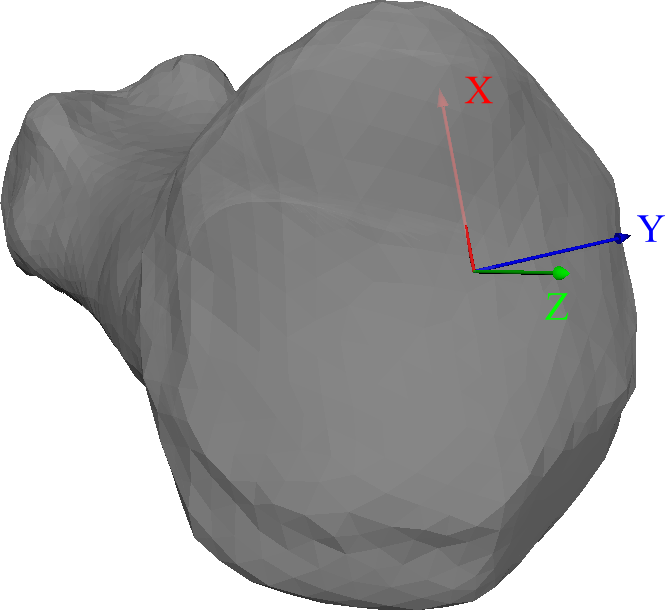
\includegraphics[width=\linewidth]{\RootDir{img/acs_mc1_2.png}}
	\end{subfigure}%%
	
	\caption[Joint Coordinate System of the TMC joint]{Examples of coordinates systems defined by \cite{halilaj_2013_thumb} and computed with our method, for the \texttt{TPM} (left) and \texttt{MC1} (right) bones of a subject.}
	\label{fig:SCS} 
\end{figure}





\subsection{Discussion}
\label{Discussion}

We have proposed a method that is able to reproduce coordinate systems for all bones of our database when one or a few examples have been defined. The method rests on the correspondence relations between the meshes. We have tested it using a joint coordinate system definition given in \cite{halilaj_2013_thumb} for the TMC joint. Systems based on this definition were computed using both their analytical method and our correspondence-based one. We prove that the steadiness of the systems are in the same range of values using both approaches, even slightly better for our procedure. Our method is completely based on the quality of the correspondence relations previously created, and gets equal results than another very specialized method. We deduce that the correspondence between meshes is to be trusted. 

We have equivalent results than a local specialized method that is fit to compute one definition of coordinate systems for one articulation only. Yet our approach uses no prerequisite that makes it specific neither to this joint nor to this particular system definition based on principal curvatures. Any system described by a user on one or a few examples can be reproduced on any bone, for instance systems that are better adapted to the TMC joint. It has indeed been proven that the principal directions of curvature of the saddle-shaped surfaces of the TMC joint are not the actual kinematic rotation axis (\cite{hollister_1992_axes}, \cite{crisco_2015_vivo}). Any other wrist joint can be examined as well. We could imagine for example to define multiple joint coordinate systems to study the entire articular chain of the thumb in the wrist, including the radius and the scaphoid as suggested by \cite{dagostino_2017_vivo}.


This mapping of bones through dense correspondence can also have other applications. For example the location of the ligaments attachment to bones can naturally be transferred from one subject to all other. Simulations of tendons adapting to various shapes of wrist bones could be imagine as a possible application. 